\chapter{REPRESENTAÇÃO GRÁFICA}

\begin{quote}
``O maior valor de uma imagem é quando ela nos força a notar o que nunca esperávamos ver.'' \\
\hfill --- \textbf{John Tukey}
\end{quote}

\begin{figure}[H]
\centering
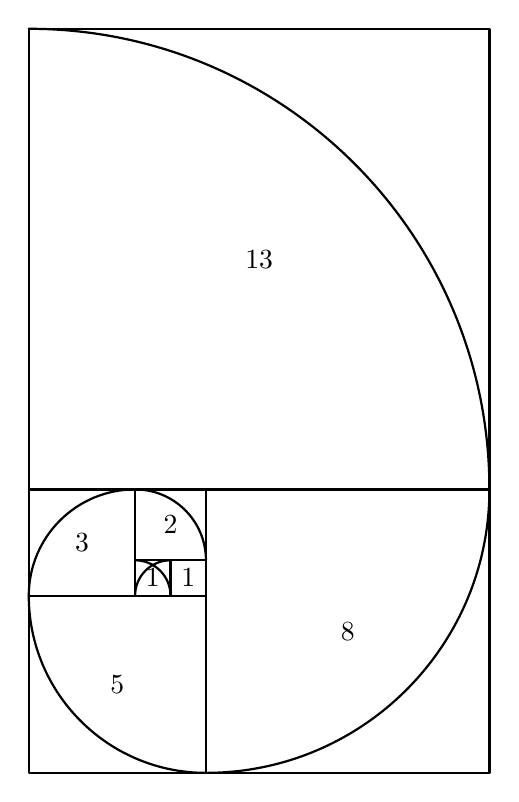
\begin{tikzpicture}[scale=0.45, line cap=round, line join=round, thick]

% ===== Quadrados de Fibonacci (tamanhos: 1,1,2,3,5,8,13) =====

% S1 (1x1)
\draw (0,0) rectangle (1,1);
\node at (0.5,0.5) {1};

% S2 (1x1) à direita de S1
\draw (1,0) rectangle (2,1);
\node at (1.5,0.5) {1};

% S3 (2x2) acima de S1+S2
\draw (0,1) rectangle (2,3);
\node at (1,2) {2};

% S4 (3x3) à esquerda do conjunto
\draw (-3,0) rectangle (0,3);
\node at (-1.5,1.5) {3};

% S5 (5x5) abaixo do conjunto
\draw (-3,-5) rectangle (2,0);
\node at (-0.5,-2.5) {5};

% S6 (8x8) à direita do conjunto
\draw (2,-5) rectangle (10,3);
\node at (6,-1) {8};

% S7 (13x13) acima do conjunto
\draw (-3,3) rectangle (10,16);
\node at (3.5,9.5) {13};

% ===== Arcos de 1/4 formando a espiral =====
\draw  (1,0) arc[start angle=0, end angle=90, radius=1];
\draw  (1,1) arc[start angle=90, end angle=180, radius=1];
\draw  (2,1) arc[start angle=0, end angle=90, radius=2];
\draw  (0,3) arc[start angle=90, end angle=180, radius=3];
\draw  (-3,0) arc[start angle=180, end angle=270, radius=5];
\draw  (2,-5) arc[start angle=270, end angle=360, radius=8];
\draw  (10,3) arc[start angle=0, end angle=90, radius=13];

\end{tikzpicture}
\caption{Espiral de Fibonacci com quadrados de lados $1,1,2,3,5,8,13$ e números nos quadrados.}
\label{fig:fibonacci_espiral_numeros}
\end{figure}


\newpage
\section{Desenvolvimento Histórico}

As origens da representação gráfica remontam aos primeiros diagramas geo\-mé\-tri\-cos, às tabelas de posição das estrelas e aos mapas. No século XVI, com a expansão marítima europeia, surgiram novos instrumentos e técnicas que possibilitaram formas mais precisas de apresentação visual do conhecimento. Até meados do século XVII, foram produzidos os primeiros mapas e diagramas sistematizados.\vskip0.3cm

Entre 1600 e 1699, período conhecido como das Medições e Teorias, os grandes desafios estavam relacionados à mensuração física do tempo, das distâncias e do espaço, sobretudo para aplicações em astronomia, navegação e expansão territorial. Nesse contexto, avançaram as estimativas, as probabilidades, a demografia e o campo nascente da estatística. Ao final desse período, já estavam consolidados os elementos necessários para o início de um pensamento visual estruturado. \vskip0.3cm

No século XVIII (1700–1799), denominado das Novas Fórmulas Gráficas, os cartógrafos passaram a representar mais do que apenas a posição geográfica, introduzindo informações relacionadas à geologia, economia, demografia e saúde.  \vskip0.3cm

O crescimento do volume de dados impulsionou novas formas de visualização. Recursos tecnológicos, como o uso de cores, a litografia e a imprensa, abriram novos caminhos para a difusão da informação. \vskip0.3cm

\newpage
Em 1786, William Playfair produziu os primeiros gráficos de linhas, barras e setores, estabelecendo bases para a infografia moderna. \vskip0.3cm


\begin{figure}
    \centering
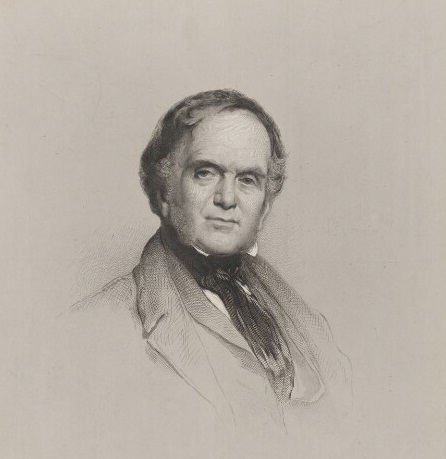
\includegraphics[scale=0.45]{figures/william_playfair.jpeg}
    \caption{William Playfair (1759-1823)}
    \label{fig:my_label4}
\end{figure}


Na primeira metade do século XIX (1800–1849), conhecida como \textbf{Início da Infografia Moderna}, houve uma verdadeira explosão na produção de gráficos estatísticos e de mapas temáticos. \vskip0.3cm

As inovações do século anterior permitiram o desenvolvimento de praticamente todas as formas de gráficos que conhecemos hoje. Na cartografia, por exemplo, mapas simples evoluíram para atlas complexos, baseados em grande variedade de dados.  
\vskip0.3cm

Entre 1850 e 1900, período denominado \textbf{Era de Ouro da Estatística}, consolidaram-se as condições para um rápido crescimento da visualização de dados. Escritórios de análises se multiplicaram na Europa, refletindo a crescente importância das informações numéricas para o planejamento social, industrial, comercial e de transporte. \vskip0.3cm

A teoria estatística desenvolvida por Gauss e Laplace forneceu os fundamentos para compreender grandes volumes de dados.  
\vskip0.3cm 

Já no início do século XX (1900 a 1949), ocorreu o chamado \textbf{Período Negro dos Gráficos Estatísticos}. 

\newpage
Nesse intervalo, poucas inovações surgiram, e o entusiasmo do século anterior foi ofuscado pela valorização crescente da quantificação e dos modelos formais. Apesar disso, os recursos gráficos disponíveis se popularizaram em áreas como governo, comércio e ciências, consolidando a visualização como instrumento essencial de comunicação científica.\vskip0.3cm 

A partir de 1975, com a expansão da informática, iniciou-se uma nova fronteira para a representação gráfica. O desenvolvimento de softwares interativos e de fácil manipulação permitiu avanços sem precedentes. \vskip0.3cm 


Nos anos 1990, com a popularização da multimídia e da internet, multiplicaram-se as formas dinâmicas de visualização, como animações, gráficos interativos e mapas em escala variável.\vskip0.3cm  


\section{Autores Importantes na Representação Gráfica}

Diversos autores contribuíram de forma decisiva para a consolidação da representação gráfica ao longo da história. Entre eles:

\begin{itemize}
\item \textbf{John Snow} (1854) – Médico britânico considerado o pai da epidemiologia moderna, identificou a fonte transmissora da cólera em Londres utilizando um mapa que registrava os locais de ocorrência dos óbitos.;
\item \textbf{Florence Nightingale} (1858) – Enfermeira britânica que produziu os famosos coxcomb diagrams, representando as baixas do exército britânico na Guerra da Crimeia;
\item \textbf{Charles Joseph Minard} (1869) – Engenheiro civil francês que retratou a dizimação do exército de Napoleão em sua campanha contra a Rússia, criando uma das mais notáveis visualizações narrativas da história.;
\item \textbf{Willard Brinton} (1914) – Engenheiro americano, autor do primeiro livro voltado à visualização de dados aplicada a negócios.;
\item \textbf{Mary Eleanor Spear} (1952) – Publicou obra com boas práticas de construção de gráficos, fruto de sua experiência no governo americano;
\item \textbf{Jacques Bertin} (1967) – Cartógrafo francês, autor de Sémiologie graphique, obra pioneira sobre teoria da visualização, propondo um sistema complexo de representação visual especialmente aplicado à cartografia;
\item \textbf{John Tukey} (década de 1970) – Matemático americano que introduziu o conceito de visualização exploratória e confirmatória, pioneiro no uso de computadores para análise gráfica.;
\item \textbf{Edward R. Tufte} (1983) – Autor de referência em design de informação, combinou rigor estatístico com princípios de clareza visual, defendendo a comunicação eficiente de ideias complexas;
\item \textbf{Jock Mackinlay} (1986) – Com sua tese de doutorado, levou os conceitos de Jacques Bertin para a era digital;
\item \textbf{Leland Wilkinson} (1999) – Estabeleceu uma gramática concisa para a descrição dos componentes de um gráfico, influenciando o desenvolvimento de ferramentas modernas de visualização.
\end{itemize}

\section{Porque usar Gráficos?}

O propósito fundamental da análise de dados é a comunicação de ideias. Em termos simples, cabe ao pesquisador analisar informações extraídas de bancos de dados e sugerir possíveis interpretações para a realidade.\vskip0.3cm


Um gráfico deve justificar a sua existência e dialogar com o público-alvo. Muitas vezes, estatísticas são mais bem compreendidas quando apresentadas graficamente do que em tabelas, pois a representação visual facilita comparações, revela tendências e evidencia relações entre variáveis.\vskip0.3cm


Embora possam fornecer menos detalhes que as tabelas, os gráficos oferecem uma visão global dos dados, permitindo identificar tendências, ocorrências excepcionais, valores mínimos e máximos, bem como ordens de grandeza.\vskip0.3cm


Os gráficos são particularmente úteis para mostrar:


\begin{itemize}
    \item \textbf{Comparação}: identificar qual item é maior ou menor;
    \item \textbf{Evoluções temporais:} visualizar como uma variável se altera ao longo do tempo;
    \item \textbf{Distribuições}: compreender a frequência ou dispersão dos valores;
    \item \textbf{Relações}: observar correlações entre variáveis;
    \item \textbf{Composição}: representar a participação relativa de cada parte em relação ao todo.
\end{itemize}


\section{Quando Pode Não ser Apropriado usar Gráficos}

%\begin{quote}
%``Um mau gráfico é pior do que nenhum gráfico.'' \\
%\hfill --- \textbf{Wallgren} (1996)
%\end{quote}

Embora sejam poderosos instrumentos de comunicação, os gráficos não são sempre a melhor escolha. Em determinadas situações, textos ou tabelas podem transmitir informações de forma mais clara e objetiva \vskip0.3cm

Deve-se reconsiderar o uso de gráficos quando os dados:

\begin{itemize}
\item Estão muito dispersos; 
\item São escassos ou apresentam poucos valores; 
\item São excessivamente numerosos, comprometendo a legibilidade; 
\item Apresentam pouca ou nenhuma variação significativa.
\end{itemize}

%\newpage
\section{Conceitos Básicos de Representação Gráfica}

Com palavras, números ou desenhos podem-se mostrar às pessoas interessadas o resultado da pesquisa, antes mesmo de aplicarem-se sobre os dados as operações matemáticas, que permitirão a interpretação final por parte da equipe encarregada do levantamento estatístico.\vskip0.3cm

A exposição por palavras é dita descritiva, a numérica é também conhecida como tabular e, finalmente, os desenhos constituem a exposição gráfica. Um relatório final reúne, quase sempre, as três modalidades de exposição, apresentando: gráficos, para ilustrar ou acentuar determinados itens: tabelas, para resumir a massa de dados observados no período de atividades; e palavras, para orientar a leitura, comentar as tabelas analisar os gráficos e concluir o relatório.\vskip0.3cm

Em muitas situações a apresentação gráfica é preferível a apresentação tabular. Os gráficos têm um impacto visual e uma facilidade de interpretação que o tornam muitas vezes mais úteis que as tabelas.\vskip0.3cm

A representação gráfica das séries estatísticas tem por finalidade representar os resultados obtidos, permitindo que se chegue a conclusões sobre a evolução do fenômeno ou sobre como se relacionam os valores da série. A escolha do gráfico mais apropriado ficará a critério do analista.\vskip0.3cm

\newpage
As representações dos dados em sua forma gráfica constituem importantes instrumentos de comunicação rápida, clara e efetiva, poupando, sobretudo, tempo e esforço na visualização de dados resumidos, permitindo fixar uma imagem duradoura, daí o largo uso dessas representações em trabalhos científicos atualmente. (Ayres, 2003).\vskip0.3cm

A estatística gráfica são representações visuais dos dados estatatísticos que devem corresponder, mas nunca substituir as tabelas estatísticas.



\section{Classificação Didática dos Gráficos}
\subsection{Quanto a Forma}

Há três tipos de gráficos, classificados quanto ao critério da forma:

\begin{enumerate}
  \item \textbf{Diagramas}: os diagramas são gráficos geométricos dispostos em duas dimensões. Os diagramas são os gráficos mais usados na representação de séries estatísticas e se  apresentam através de uma grande variedade de tipos.
  \item \textbf{Cartogramas}: os cartogramas são ilustrações relativas a cartas geográficas, largamente difundidas em Geografia, História e Demografia.
  \item \textbf{Estereogramas}: os estereogramas representam volumes e são apresentados em três dimensões. Muitas vezes são confeccionados em cartolinas ou madeira quando não desenhados em perspectiva.
\end{enumerate}

\subsection{Quanto ao Objetivo e Uso}

É possível distinguir, de certo modo arbitrariamente, dois objetivos que justificariam o emprego de gráficos. Os gráficos são usados para apresentar visualmente dados numéricos, proporcionando maior facilidade e rapidez de compreensão dos mesmos, ou, então, para apresentar conclusões ou resultados de uma análise. Há portanto, dois tipos de gráficos, conforme o objetivo ou uso a que se destinam: gráficos de informações e gráficos de análise.


\newpage
\subsubsection{Gráfico de Informação}

São gráficos destinados principalmente ao público em geral, objetivando proporcionar uma visualização rápida e clara da intensidade das modalidades e dos valores relativos ao fenômeno observado. São gráficos tipicamente expositivos, devendo, por conseguinte, ser o mais o completo possível, dispensando comentários explicativos adicionais. Nos gráficos de informação não se deve prescindir dos títulos. Já as legendas podem ser omitidas, desde que as informações desejadas  estejam presentes, possibilitando a completa interpretação do gráfico.



\subsubsection{Gráfico de Análise}

Os gráficos de análise prestam-se melhor ao trabalho estatístico, fornecendo elementos úteis à fase de análise dos dados, sem deixar se ser também informativos. Quando se usam gráficos para apresentar os resultados de uma análise, esses freqüentemente vêm acompanhados de uma tabela. Inclui-se, muitas vezes, um texto dissertativo, chamando a atenção do leitor para os pontos principais revelados pelo gráfico ou pela tabela. Muitos relatórios administrativos, econômicos ou de qualquer outra natureza combinam as três formas de apresentação de dados. Isto porque, na prática, poucas pessoas têm habilidade com números, e as que têm dificuldades consultarão, via de regra, apenas o gráfico. Por outro lado, a maior parte das pessoas nunca examinará as tabelas estatísticas, preferindo analisar os gráficos e eventualmente procurar no texto a informação adicional necessária.\vskip0.3cm



\section{Elementos  Básicos na Construção de Gráficos}

Assim como tabelas, os gráficos devem ser referenciados no texto. Se eles ocorrem em um trabalho, é porque possuem alguma importância, fornecem alguma informação. Portanto, eles precisam ter alguma explicação ou comentário a respeito deles no corpo do trabalho.\vskip0.3cm 

A representação gráfica deve conter determinados elementos que são essenciais para a sua compreensão, sendo esses elementos:

\newpage
\subsection{Elementos Básicos}

\begin{itemize}
\item \textbf{Número}: utilizado para identificar o gráfico no texto, sendo sempre precedido da palavra GRÁFICO com o seu número. Por exemplo: GRÁFICO 1, GRÁFICO 2 etc, ou de acordo com a numeração do capítulo, GRÁFICO 1.1, GRÁFICO 1.2, e assim por diante. \item \textbf{Título}: deve conter designação do fenômeno observado (O QUE?) e o local (ONDE?) e data de ocorrência do mesmo (QUANDO?) e (COMO?), ficando abaixo do gráfico. 


O título deve preferencialmente ser escrito após o número do gráfico, devendo ser separado por espaço, hífen e espaço em letras maiúsculas seguindo o padrão do texto. O título deve estar presente em qualquer tipo de representação gráfica a ser escrito com vista a orientar o leitor na sua interpretação. Simultaneamente, deve ser conciso, relevante e claro, ou seja, conter apenas informação essencial para uma interpretação correta do gráfico. 
\item \textbf{Fonte}: indicação do órgão ou entidade responsável pelo fornecimento dos dados usados na elaboração do gráfico. Utilizar letras maiúsculas para escrever FONTE, devendo ser seguida de dois pontos, espaço e o nome da fonte utilizada. Quando os dados foram obtidos pelo próprio autor, por exemplo, em uma pesquisa e campo, a fonte pode ser escrita como: FONTE: o autor. 
\item \textbf{Nota}: quando necessária, é utilizada para a apresentação de informações de natureza geral, esclarecendo o conteúdo ou metodologia utilizada. A nota vem em seguida à fonte. A palavra NOTA deve ser escrita em letras maiúsculas, devendo ser seguida de dois pontos, espaço e a explicação da nota. 
\item \textbf{Nota Específica}: quando necessária, é utilizada para esclarecer dados sobre um item ou uma parte específica do gráfico; empregam-se chamada, indicadas no gráfico, geralmente no titulo ou na legenda. A nota específica deve ser chamada por algarismos arábicos entre parênteses.

\newpage
\item \textbf{Legenda}: a legenda é constituída por símbolos e respectivas designinações. O procedimento dos sinbolos (cor ou outros) deve ser realizado de modo a que não haja lugar para qualquer confusão visual entre eles e, consequentemente, para que exista uma ligação clara entre os simbolos e a componente representada. As desiginações, por seu lado, devem ser claras e concisas, deixando para notas adjascentes eventuais esclarecimentos. Os símbolos devem aparecer na mesma ordem que as respectivas componentes: horizontalmente quando estão lado a lado e verticalmente quando estão umas sobre as outras (WALLGREN, 1996). Uma boa legenda deve fazer mais do que simplesmente etiquetar as componentes do gráfico. Deve dizer-nos o que é importante e qual é o objetivo do gráfico:   
informar o leitor e obrigar quem faz o gráfico a estruturar a informação (CLEVELANDO e MCGILL, 1984a).
\item \textbf{Escalas}: Em um gráfico, as informações que possuem uma escala devem ser apresentadas com clareza. Os números da escala devem estar na posição horizontal e na região externa dos eixos. A unidade de medida deve aparecer no final de cada linha do gráfico. Caso não seja possível apresentar a escala por completo, pode-se fazer um corte no eixo correspondente para informar que a escala não está completa.


\item \textbf{Linhas Auxiliares}: um dos elementos gráficos visualmente mais mo\-nó\-to\-nos são as linhas auxiliares. devem, por isso ser suprimidas ou abafadas de tal forma que sua presença se torne implícita. Ainda que possam auxiliar a leitura dos dados, a maioria das linhas auxiliares escuras tem um grande peso visual, encobrindo muitas vezes, o mais importante do gráfico: a informação. Quando foram realmente necessárias deve-se optar por usar uma cor neutra e, no caso particular de um fundo branco, a cor cinzenta. Em certos caos em particular nas séries temporais, pode ser considerado importante incluir linhas auxiliares verticais como auxilio a leitura de valores por forma a complementar a leitura evolutiva da série com a leitura de valores em particular. Na maioria dos gráficos de séries temporais, os dados mais recentes estão situados à direita e longe das identificações do eixo dos valores, normalmente localizados à esquerda, fazendo com que o olho humano tenha que se movimentar alternadamente entre os dados e os valores ao longo das margens do gráfico. 
\newpage
Esta imprecisão na leitura pode ser atenuada posicionando o eixo à direita junto dos dados mais recentes, duplicando o eixo, ou posicionando os valores junto das coordenadas respectivas (TUFTE, 198).\vskip0.3cm

Os gráficos com dois eixos distintos são normalmente utilizados quando se têm diferentes unidades de medida ou existem diferenças consideráveis de valores nas categorias de uma variável. Este tipo de gráficos deve ser evitado dado que é normalmente de difícil interpretação e, em muitos casos, bastante confuso (SCHMID, 1992). Por princípio, deve privilegiar-se a escala completa (com início em zero ou noutro valor de referência) em nome da honestidade na apresentação. Contudo, essa quebra é admissível nos casos em que a informação apresenta pequenas variações, desde que acompanhada por uma simbologia perceptível ao leitor. Para melhor compreender os dados na fase da análise exploratória não existe qualquer problema em manipular as escalas e extrapolar eventuais variações, mas na fase da divulgação, deve existir algum cuidado para não evidenciar graficamente alterações nos dados que na verdade não ocorreram. A quebra de escala é um exemplo de como se pode distorcer a mensagem transmitida. Quando o efeito nos dados é significativamente. 
\end{itemize}

Quando se representa as informações de qualquer tipo de estudo em forma gráfica, precisam-se fazer algumas perguntas, tais como (VERGNAUD, 1987) e (WALLGREEN, 1996):

\begin{itemize}
\item Representar O Que? Para Quê?
\item Um gráfico Realmente é a Melhor Opção?
\item Qual é o Público Alvo?
\item Qual é o Objetivo do Gráfico?
\item Que Tipo de Gráfico Deve Ser Usado?
\item Como o Gráfico Deve Ser Apresentado?
\item Que Tamanho o Gráfico Deve Ter?
\item Deverá Ser Usado Apenas Um Gráfico?
\item A Qual Meio Técnico Se Deve Recorrer?
\end{itemize}

Wallgreen(1996) acrescenta que a utilização gráfica apenas se pode consumar após serem formuladas, e convenientemente respondidas, as seguintes perguntas:

\begin{itemize}
\item O Gráfico é Fácil de Ler? 
\item O Gráfico Pode Ser Mal Interpretado? 
\item O Gráfico Tem o Tamanho e a Forma Certa? 
\item O Gráfico está Localizado no Local Certo? 
\item O Gráfico Beneficia por Ser Colorido? 
\item A Compreenção do Gráfico Foi Testada com Alguém?
\end{itemize}



\section{Requisitos Fundamentais de uma Representação Gráfica}

A representação gráfica de um fenômeno deve obdecer a certos requisitos fundamentais para serem úteis.

\begin{enumerate}

\item \textbf{Compreensível}: permite visualizar as relações entre variáveis.
\item \textbf{Necessidade}: um gráfico deve ser útil para representar dados, deve haver uma necessidade para inserir elementos em um gráfico.
\item \textbf{Confiabilidade}: os dados devem estar corretamente representados, principalmente no que diz respeito a escala.
\item \textbf{Simplicidade}: deve ser destituída de detalhes de importância secundária, assim como de traço desnecessários que possam levar o observador a uma análise morosa ou com erros, ou seja, a uma interpretação equivocada do fenômeno em estudo. 
\item \textbf{Clareza}: deve possibilitar uma correta interpretação dos valores representativos do fenômeno em estudo. 
\item \textbf{Veracidade}: deve expressar a verdade sobre o fenômeno em estudo.
\end{enumerate}

\section{Diretrizes e Recomendações para a Construção de um Gráfico}

\begin{itemize}
\item O título do gráfico deve ser o mais claro e completo possível. Quando necessário, deve-se acrescentar subtítulos;
\item A orientação geral dos gráficos deve ser da esquerda para a direita;
\item As quantidades devem ser representadas por grandezas lineares;
\item Sempre que possível, a escala vertical há de ser escolhida de modo a aparecer a linha 0 (zero);
\item Só devem ser incluídas no desenho as coordenadas indispensáveis para guiar o olhar do leitor ao longo da leitura. Um tracejado muito cerrado dificulta o exame do gráfico;
\item A escala horizontal deve ser lida da esquerda para a direita, e a vertical de baixo para cima;
\item Os títulos e marcações do gráfico devem ser dispostos de maneira que sejam facilmente lidos, partindo da margem horizontal inferior ou da margem esquerda.
\item Um gráfico deve induzir o observador a pensar sobre o conteúdo e não no desenho do gráfico, na tecnologia ou outros atributos.
\item Induzir que os olhos do observador comparem diferentes partes dos dados.
\item Revelar diferentes detalhes dos dados, desde a perspectiva global até detalhes particulares (MAKINLAY, 1986).
\item Ter um objetivo bastante claro: descrição, exploração, tabulação e decoração.
\item Utilize uma linha de referência quando há algum valor importante que deva ser visto em todo o gráfico, por exemplo, uma linha média. Cuide para que isso não interfira na apresentação do gráfico.
\item Elimine da visualização gráficos e textos desnecessários. Uma boa medida de
quantos elementos são desnecessários em uma figura é a quantidade de tinta ou de
pixels gastos com itens que não são dados de interesse.
\item Explore a utilização de símbolos e de atributos visuais que facilitem a percepção
dos dados e dos padrões existentes nos mesmos.
\end{itemize}


\section{Sugestões de Leitura e Interpretação de um Gráfico}

\begin{itemize}
\item Declarar qual o fenômeno ou fenômenos representados, a região considerada, o período de tempo, a fonte dos dados, etc;
\item Examinar o tipo de gráfico escolhido, verificar se é o mais adequado, criticar a sua execução, no conjunto e nos detalhes;
\item Analisar cada fenômeno separadamente, fazendo notar os pontos mais em evidência, o máximo e o mínimo, assim como as mudanças mais bruscas; \item Investigar se há uma "tendência geral" crescente ou decrescente ou, então, se o fato exposto é estacionário; 
\item Procurar descobrir a existência de possíveis ciclos periódicos, qual o período aproximado, etc. 
\item Quando um gráfico for inserido em um texto, recomenda-se que este seja destacado tanto do texto que o precede, como do texto imediamente subsequente, por meio de três espaços simples. \item Com relação a variação das cores num mesmo gráfico é recomendada para o caso de gráficos comparativos, dos quais, se dá preferência a pouca variação de cores.
\end{itemize}

O verdadeiro desafio é saber apresentar os dados de forma interessante e atrativa. Contudo, construir gráficos e mapas estimulantes e cientificamente corretos não é tarefa tão fácil como pode parecer. Não basta ter os dados e saber usar os programas informáticos. É preciso saber transformá-los numa história bem contada e transmitir idéias e fenômenos que dificilmente seriam visíveis de outra forma.

\newpage
\section{Principais Erros Encontrados em um Gráfico}

Os problemas mais comuns que podem comprometer a efetividade de uma visualização gráfica são:


\begin{itemize}
\item Em geral o excesso de decoração é um problema.
\item Ausência ou erro na escala de eixos.
\item Ausência de um título, marcas e indicadores.
\item Não Colocar dados suficientes na visualização de forma a contextualizar as informações mais relevantes apresentadas.
\item Excesso de informação.
\item  Utilizar gráficos sobrepostos em escalas diferentes ou com sistemas de coordenadas distintos, o que impede uma comparação justa entre os dados.
\item Não fazer um mapeamento dos dados para marcas e atributos visuais de forma adequada.
\end{itemize}

\newpage
\section{Tipos de Gráficos}
\subsection{Ramo-e-Folhas (\textit{Stem and Leaf})}

O diagrama de \textbf{Ramo-e-Folhas}, também conhecido como
\textbf{Talo-e-Folha}, \textbf{Caule-e-Folha} ou, em inglês,
\textit{Stem and Leaf}, foi proposto em 1977 pelo estatístico
americano \textbf{John Wilder Tukey}.  \vskip0.3cm

Esse tipo de representação gráfica constitui uma ferramenta simples,
porém extremamente útil, para organizar observações numéricas de forma
estruturada, permitindo uma visualização rápida da distribuição dos dados. \vskip0.3cm

Uma das principais vantagens do diagrama de ramo-e-folhas é que,
diferentemente do histograma, ele preserva os valores originais da amostra,
ou seja, os dados podem ser reconstruídos a partir do gráfico.
Por essa razão, ele pode ser utilizado tanto como uma apresentação direta
dos dados quanto como uma etapa preliminar na construção de tabelas de frequência. \vskip0.3cm

A Tabela~\ref{febreamarela} apresenta um conjunto de dados brutos referentes
ao número de doses aplicadas mensalmente da vacina contra febre amarela,
no município de Belém (PA), ao longo dos últimos anos.


\begin{table}[H]
    \centering
    {
\caption{Doses de Vacinas sobre Febre Amarela, aplicadas mensal nos últimos 5 anos no muncípio de Belém, Estado do Pará - 2024 \textbf{(Dados Brutos)}.}
    \label{febreamarela}
    \vspace{0.1cm}
\begin{tabular}{c|c|c|c|c|c|c|c}
  \hline \hline
  196 & 221 & 183 & 186 & 121 & 181 & 180 & 143  \\
  200 & 154 & 153 & 174 & 120 & 168 & 167 & 141  \\
  245 & 228 & 174 & 199 & 181 & 158 & 176 & 110  \\
  193 & 131 & 154 & 115 & 160 & 208 & 158 & 133  \\
  207 & 180 & 190 & 193 & 194 & 133 & 156 & 123  \\
  134 & 178 &  76 & 167 & 184 & 135 & 229 & 146  \\
  218 & 157 & 101 & 171 & 165 & 172 & 158 & 169  \\
  199 & 151 & 142 & 163 & 145 & 171 & 148 & 158  \\
  160 & 175 & 149 & 201 & 160 & 237 & 150 & 135  \\
  105 & 87  & 97  & 176 & 150 & 170 & 118 & 149  \\
\hline \hline
\end{tabular}}
\\
\hspace{-3.5cm} Fonte: SESMA-PA, 2022.
\end{table}

\newpage
Para construir um diagrama de ramo-e-folhas, cada observação numérica é
decomposta em duas partes principais:

\begin{itemize}
    \item o \textbf{ramo}, formado pelos primeiros dígitos do valor;
    \item a \textbf{folha}, formada pelo dígito final, que completa a observação.
\end{itemize}

Os ramos são dispostos em ordem crescente no lado esquerdo de uma linha vertical,
enquanto as folhas correspondentes são registradas à direita.
Opcionalmente, pode-se adicionar uma coluna com a frequência de cada ramo,
facilitando a interpretação quantitativa. \vskip0.3cm


A Tabela~\ref{ramosfolhas} apresenta o diagrama de ramo-e-folhas construído
para os dados da vacina contra febre amarela.

\newpage
\begin{table}[h]
    \centering
    {
    \caption{Diagrama de Ramo-e-Folhas para as Doses de Vacinas sobre Febre Amarela, aplicadas nos ultimos 5 anos no muncípio de Belém, Estado do Pará - 2024.}
    \label{ramosfolhas}
    \vspace{0.1cm}
\begin{tabular}{c|l|c}
\hline \hline
\textbf{Ramo} & \textbf{Folhas} & \textbf{Frequência} \\
\hline \hline 
 7  &  6                                   & 1  \\
 8  &  7                                   & 1  \\
 9  &  7                                   & 1  \\
 10 &  5, 1                                & 2  \\
 11 &  5, 8, 0                             & 3  \\
 12 &  1, 0, 3                             & 3  \\
 13 &  4, 1, 3, 5, 3, 5                    & 6  \\
 14 &  2, 9, 5, 8, 3, 1, 6, 9              & 8  \\
 15 &  4, 7, 1, 3, 4, 0, 8, 8, 6, 8, 0, 8  & 12 \\
 16 &  3, 0, 7, 3, 0, 5, 0, 8, 7, 9        & 10 \\
 17 &  8, 5, 4, 4, 1, 6, 2, 1, 0, 6        & 10 \\
 18 &  0, 3, 6, 1, 4, 1, 0                 & 7  \\
 19 &  9, 6, 0, 9, 3, 4                    & 6  \\
 20 &  7, 1, 0, 8                          & 4  \\
 21 &  8                                   & 1  \\
 22 &  1, 8, 9                             & 3  \\
 23 &  7                                   & 1  \\
 24 &  5                                   & 1  \\
 \hline
 Total   &                                 & 80 \\ 
 \hline \hline
\end{tabular}}
\end{table}




%----------------------------------------------------------------------------------------------------------%
\newpage
\subsection{Histogramas}

O \textbf{histograma} é um dos gráficos mais utilizados em Estatística
para representar a distribuição de frequências de uma variável quantitativa.
Trata-se de um gráfico formado por barras (retângulos) em que:

\begin{itemize}
    \item o eixo horizontal representa os \textbf{intervalos de classe}
    (ou faixas de valores da variável);
    \item o eixo vertical representa as \textbf{frequências}
    (absolutas ou relativas) associadas a cada classe.
\end{itemize}

\vskip0.3cm

Diferentemente do gráfico de barras utilizado para variáveis qualitativas,
no histograma as barras são desenhadas \textbf{justapostas}, isto é,
sem espaçamento entre elas, pois os intervalos de classe são contínuos e
adjacentes.

\vskip0.3cm

Formalmente, um histograma é construído a partir de um conjunto de
\textbf{retângulos} cujas bases estão sobre o eixo horizontal e cujas alturas
são proporcionais às frequências observadas em cada classe.
Cada retângulo possui:

\begin{itemize}
    \item \textbf{base} igual à amplitude do intervalo de classe;
    \item \textbf{altura} proporcional à frequência correspondente.
\end{itemize}
\vskip0.3cm

Em geral, a variável de interesse é apresentada no eixo $x$,
enquanto o número (ou porcentagem) de observações aparece no eixo $y$.
Alguns softwares estatísticos podem inverter essa orientação,
mas a interpretação permanece a mesma. \vskip0.3cm

Quando todas as classes possuem a mesma amplitude $h$,
a altura de cada retângulo torna-se numericamente igual à frequência da classe.
Assim, pode-se resumir:

\[
\text{Largura do retângulo} = h,
\qquad
\text{Altura do retângulo} = f,
\]

onde $f$ representa a frequência associada ao intervalo considerado. \vskip0.3cm


\newpage
O histograma permite identificar rapidamente características importantes
da distribuição dos dados, tais como: concentração de valores; dispersão; assimetria; presença de valores extremos. \vskip0.3cm

A Figura~\ref{fig:my_label25} apresenta um exemplo de histograma construído
a partir das idades de vítimas fatais em acidentes de trânsito registrados
no município de Belém no ano de 2024.

\begin{figure}[H]
    \centering
    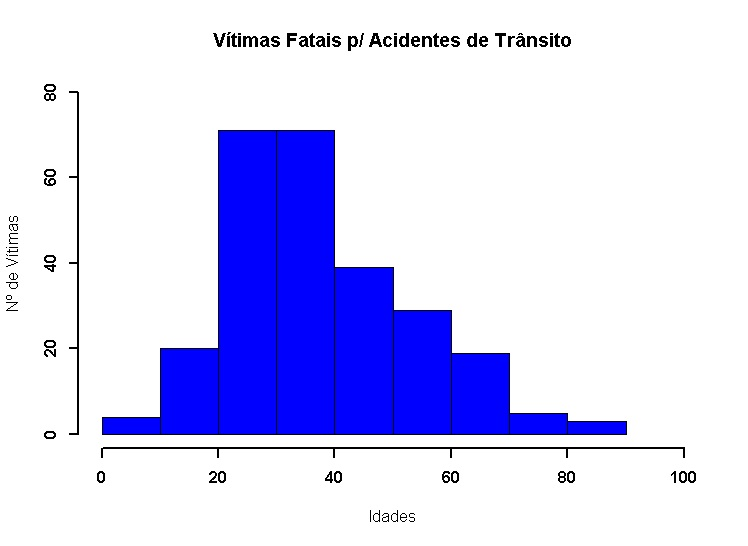
\includegraphics[scale=0.5,width=11cm]{figures/histograma1.jpeg}
    \caption{Histograma das idades de vítimas fatais em acidentes de trânsito,
    Belém (2024).}
    \label{fig:my_label25}
\end{figure}

%----------------------------------------------------------------------------------------------------------%


\newpage
\subsection{Polígono de Frequência Simples e Acumulado}

O \textbf{polígono de frequência} é um gráfico de linhas utilizado
para representar a distribuição de frequências de uma variável quantitativa.
Ele é construído a partir dos pontos médios dos intervalos de classe,
sobre os quais são marcadas as frequências correspondentes. \vskip0.3cm

Para traçar o polígono, procede-se da seguinte forma:

\begin{itemize}
    \item determina-se o ponto médio de cada classe;
    \item marca-se, sobre a perpendicular levantada nesse ponto,
    a frequência da classe;
    \item liga-se os pontos consecutivos por segmentos de reta.
\end{itemize}
\vskip0.3cm

Esse gráfico é especialmente útil para visualizar o comportamento geral
da distribuição e comparar diferentes conjuntos de dados de maneira mais clara
do que no histograma. \vskip0.3cm

\subsubsection{Polígono de Frequência Acumulada (Ogiva)}

Quando se deseja representar as \textbf{frequências acumuladas},
utiliza-se o chamado \textbf{polígono de frequência acumulada},
mais conhecido como \textbf{ogiva} ou \textbf{Ogiva de Galton}.
\vskip0.3cm

A ogiva é construída marcando-se as frequências acumuladas nos pontos
correspondentes aos \textbf{limites superiores} dos intervalos de classe.
Em seguida, esses pontos são ligados por segmentos de reta,
formando uma curva crescente. \vskip0.3cm

Esse tipo de gráfico permite responder questões importantes, tais como:

\begin{itemize}
    \item qual proporção dos dados encontra-se \textbf{até} determinado valor;
    \item qual parcela da população está \textbf{acima} de certo limite;
    \item estimativas aproximadas de percentis e medianas.
\end{itemize}
\vskip0.3cm

Além disso, a partir da ogiva é possível realizar uma
\textbf{interpolação linear}, estimando valores de frequência acumulada
para pontos situados dentro de qualquer intervalo utilizado na construção
da distribuição em classes. \vskip0.3cm

%Portanto, a ogiva constitui uma ferramenta gráfica fundamental para o estudo
%da distribuição acumulada dos dados, sendo amplamente aplicada em análises
%estatísticas descritivas.


\newpage
\vspace{-1cm}
\begin{figure}[H]
    \centering
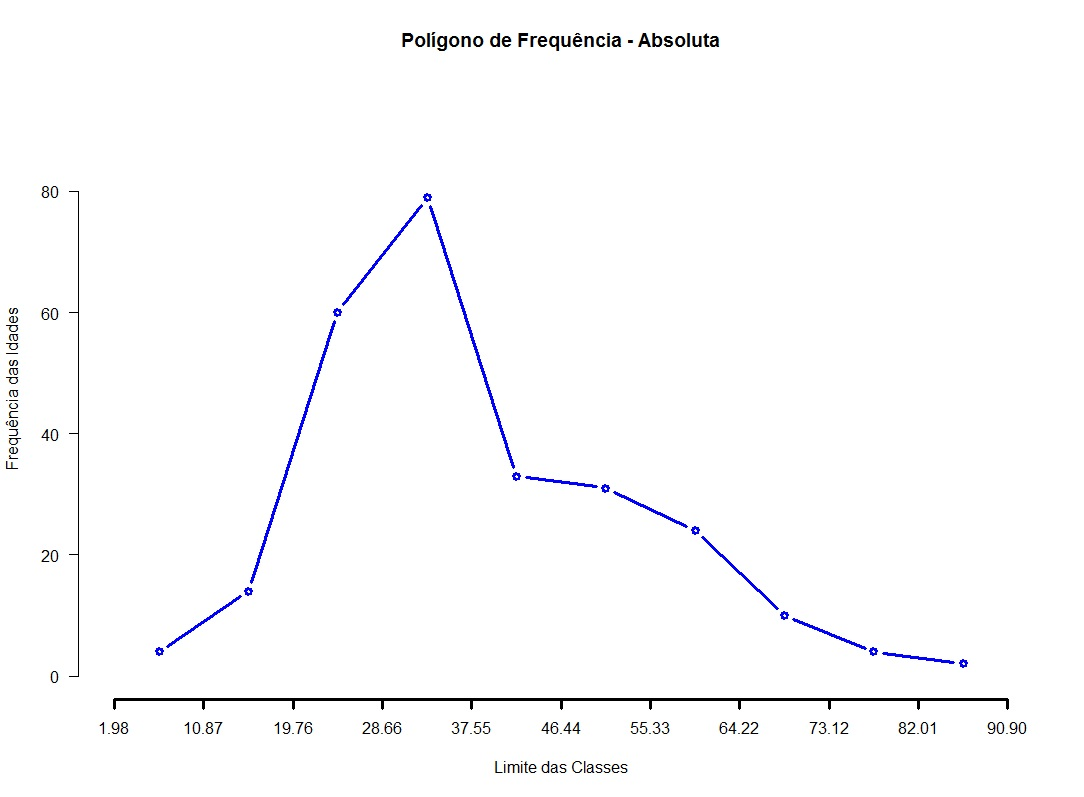
\includegraphics[scale=0.3,height=220pt,width=15cm]{figures/poligono1.jpeg}
\caption{\textbf{(Polígono de Frequências Absoluta):} das Idades de Vítimas Fatais por Acidentes de Trânsito, Belém em 2024.}
   \label{fig:my_label25}
\end{figure}
\vspace{-0.8cm}
\begin{figure}[H]
    \centering
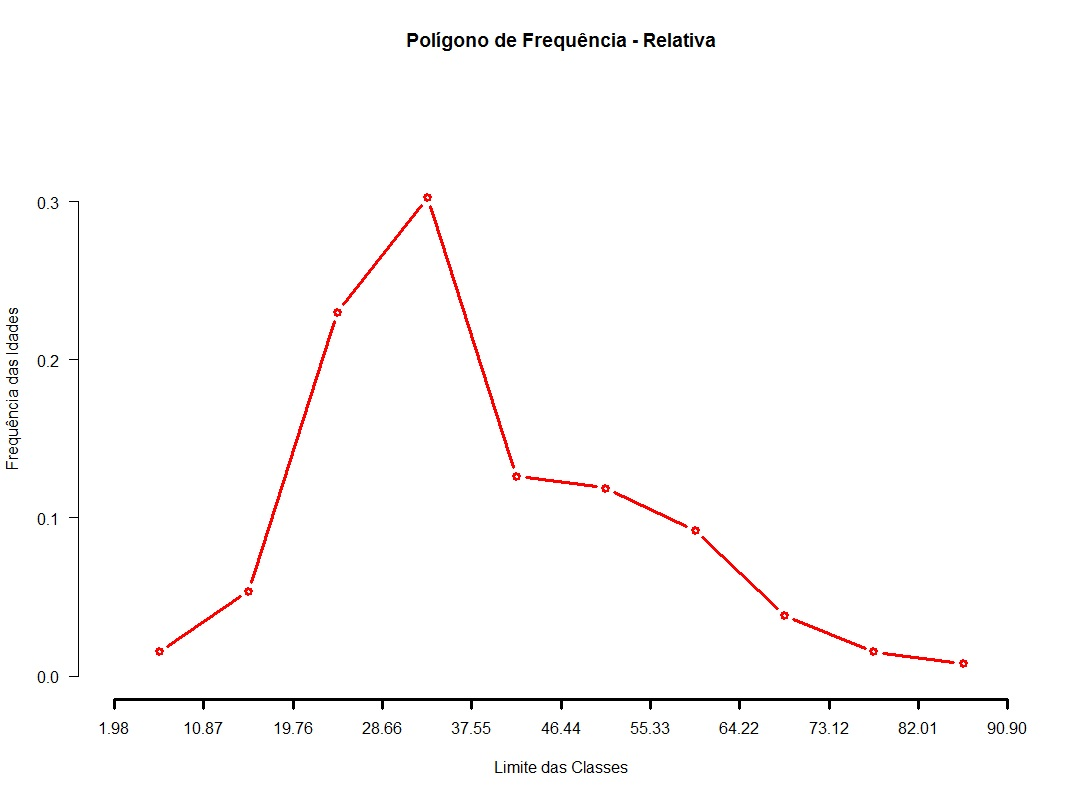
\includegraphics[scale=0.3,height=220pt,width=15cm]{figures/poligono2.jpeg}
    \caption{\textbf{(Polígono de Frequências Relativa):} das Idades de Vítimas Fatais por Acidentes de Trânsito, Belém em 2024.}
    \label{fig:my_label25}
\end{figure}


%------------------------------------------------------------------------------------------------------%
\newpage
\subsection{Gráfico de Barras}

O \textbf{gráfico de barras} é uma das representações mais utilizadas em
Estatística Descritiva, pois permite comparar categorias de forma rápida e
intuitiva. Ele é formado por dois eixos perpendiculares: um eixo horizontal,
no qual são apresentadas as \textbf{categorias} da variável, e um eixo vertical,
no qual é indicada a \textbf{frequência} (absoluta ou relativa) ou outra medida
associada a cada categoria. \vskip0.3cm

As barras devem possuir \textbf{largura constante} e serem desenhadas com
\textbf{espaçamento uniforme}, de modo a não induzir interpretações equivocadas.
A \textbf{altura} (ou comprimento, caso as barras sejam horizontais) é
proporcional ao valor representado, permitindo comparações diretas entre as
categorias. \vskip0.3cm

Os gráficos de barras são especialmente indicados para:

\begin{itemize}
    \item variáveis \textbf{qualitativas} (nominais ou ordinais), como sexo,
    cor, categoria profissional, tipo de ocorrência etc.;
    \item variáveis \textbf{quantitativas discretas}, como número de filhos,
    quantidade de veículos, número de atendimentos, entre outras;
    \item comparação entre grupos ou subgrupos, quando se deseja analisar
    diferenças entre categorias.
\end{itemize}
\vskip0.3cm

\subsubsection{Gráfico de Barras Simples}

No \textbf{gráfico de barras simples}, cada categoria é representada por uma
única barra, sendo adequado quando se deseja visualizar apenas uma distribuição
de frequências ou uma variável categórica isolada. \vskip0.3cm

\subsubsection{Gráfico de Barras Múltiplas (ou Agrupadas)}

No \textbf{gráfico de barras múltiplas}, cada categoria é representada por um
\textbf{conjunto de barras} lado a lado, geralmente correspondendo a diferentes
grupos (por exemplo: masculino/feminino, anos diferentes, regiões distintas).
Esse formato é útil para comparações simultâneas, desde que o gráfico mantenha
boa legibilidade. \vskip0.3cm


\newpage
\subsubsection{Boas práticas e cuidados na interpretação}

Apesar de serem simples, os gráficos de barras exigem alguns cuidados para
evitar distorções visuais e interpretações incorretas:

\begin{itemize}
    \item \textbf{Evitar quebras de escala:} em gráficos de barras, não se deve
    interromper o eixo vertical, pois isso pode exagerar diferenças pequenas e
    induzir o leitor ao erro;
    \item \textbf{Valores negativos:} a presença de valores negativos não é
    comum em distribuições de frequência. Quando for necessário representar
    valores positivos e negativos, recomenda-se atenção especial à escala e à
    linha de referência no zero;
    \item \textbf{Ordenação das categorias:} dependendo do objetivo da análise,
    pode ser interessante ordenar as categorias em ordem crescente ou decrescente,
    facilitando a identificação de padrões. Em outros casos, a ordenação
    alfabética pode ser adequada, principalmente em listas extensas;
    \item \textbf{Comparações consistentes:} quando dois ou mais gráficos
    representam o mesmo conjunto de categorias, a ordem das categorias deve ser
    mantida em todos eles. Além disso, recomenda-se manter a mesma escala para
    possibilitar comparações visuais corretas.
\end{itemize}

Quando existe uma categoria que agrupa valores residuais, como \textit{Outros},
é recomendável apresentá-la ao final do gráfico, evitando que ela interfira na
interpretação das categorias principais. Além disso, caso se utilize cores para
diferenciar categorias, essa classe agregada deve ser representada de forma
neutra, pois normalmente não constitui o foco principal da análise. \vskip0.4cm

Por fim, para construir um gráfico de barras de maneira adequada, é necessário
organizar os dados previamente em estruturas apropriadas, como tabelas de
frequência, vetores ou matrizes, dependendo do software estatístico utilizado.

%%%%%%%%%%%%%%%%%%%%%%%%%%%%%%%%%%%%%%%%%%%%%%%%%%%%%%%%%%%%%%%%%%%%%%%%%%%%%%%%%%%%%%%%%%
%\begin{figure}[H]
%    \centering
%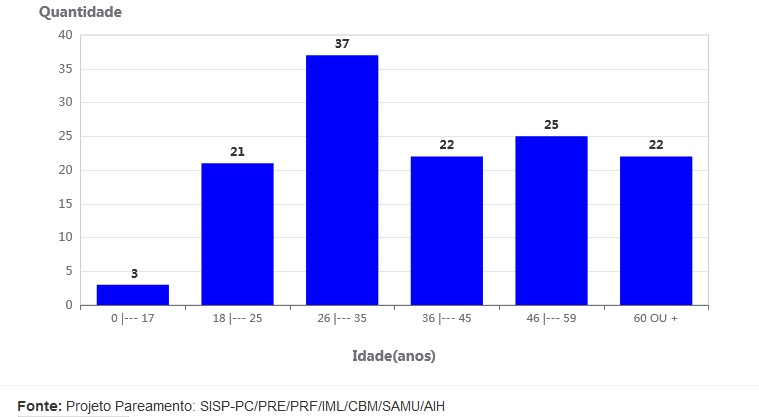
\includegraphics[scale=0.5,height=200pt,width=14cm]{figures/plot_barra1.jpg}
%    \caption{\textbf{(Gráfico de Barra):} Faixa Etária das Vítimas Fatais de Belém em 2024.}
%    \label{fig:my_label600}
%\end{figure}
%%%%%%%%%%%%%%%%%%%%%%%%%%%%%%%%%%%%%%%%%%%%%%%%%%%%%%%%%%%%%%%%%%%%%%%%%%%%%%%%%%%%%%%%%%


%------------------------------------------------------------------------------------------------------%
\newpage
\subsection{Gráfico de Linhas, Curvas ou Segmentos}

O \textbf{gráfico de linhas} (também chamado de gráfico de curvas ou de
segmentos) é um dos formatos mais utilizados para representar a evolução de
uma variável ao longo do tempo. Ele é especialmente adequado para descrever
\textbf{séries históricas} ou \textbf{séries temporais}, isto é, conjuntos de
observações registradas em instantes sucessivos.

\vskip0.3cm

Nesse tipo de gráfico, os valores da variável são marcados em um sistema de
eixos cartesianos e ligados por segmentos de reta, formando uma linha
contínua. Assim, torna-se possível visualizar de maneira clara o comportamento
global da série, identificando padrões de crescimento, queda ou estabilidade.

\vskip0.4cm

O gráfico de linhas é indicado principalmente quando:

\begin{itemize}
    \item deseja-se analisar a \textbf{tendência} de uma variável ao longo do tempo;
    \item há um número razoável de observações (em geral, cinco ou mais pontos);
    \item o objetivo é destacar a \textbf{evolução contínua} de um fenômeno.
\end{itemize}

\vskip0.3cm

Quando há poucos valores a serem comparados, gráficos de colunas ou barras
podem ser mais apropriados, pois oferecem melhor distinção visual entre
categorias isoladas.

\vskip0.5cm

\subsubsection{Aspectos históricos}

Os primeiros registros de representações gráficas datam de períodos muito
antigos, porém o uso sistemático de gráficos estatísticos ganhou força apenas
no final do século XVIII. O economista e engenheiro escocês
\textbf{William Playfair} é considerado um dos pioneiros na divulgação de
gráficos de linhas aplicados a dados econômicos, contribuindo decisivamente
para a popularização desse recurso na análise estatística.

\vskip0.3cm

Além disso, a consolidação do sistema de coordenadas cartesianas, introduzido
por \textbf{René Descartes} em 1637, estabeleceu a base matemática necessária
para relacionar equações e representações geométricas, permitindo que curvas e
linhas se tornassem ferramentas essenciais na visualização de dados.

\vskip0.5cm

\subsubsection{Interpretação e leitura de séries temporais}

A leitura de um gráfico de linhas geralmente segue duas lógicas principais:

\begin{itemize}
    \item \textbf{Avaliação da tendência geral:} identificar se a série apresenta
    comportamento crescente, decrescente ou aproximadamente constante.

    \item \textbf{Identificação de variações relevantes:} observar períodos em que
    ocorreram os maiores aumentos ou reduções, bem como pontos de inflexão,
    isto é, momentos em que a tendência se altera.
\end{itemize}
\vskip0.3cm

Em algumas situações, pode ser útil utilizar uma \textbf{escala logarítmica},
especialmente quando se deseja comparar séries cujos valores apresentam ordens
de grandeza muito diferentes. Nesse caso, embora a leitura direta dos valores
se torne menos intuitiva, a comparação proporcional entre séries é facilitada.
\vskip0.3cm

Embora o gráfico de linhas seja extremamente eficiente para representar
tendências e evolução temporal, em certos contextos pode ser mais adequado
utilizar gráficos de barras ou gráficos de área, sobretudo quando se deseja
destacar volumes acumulados ou comparar categorias discretas.
\vskip0.3cm

Assim, a escolha do tipo de gráfico deve sempre considerar a natureza dos
dados e o objetivo principal da análise estatística.



\newpage
%%%%%%%%%%%%%%%%%%%%%%%%%%%%%%%%%%%%%%%%%%%%%%%%%%%%%%%%%%%%%%%%%%%%%%%%%%%%%%%%%%%%%%%%%%
%\begin{figure}[H]
%    \centering
%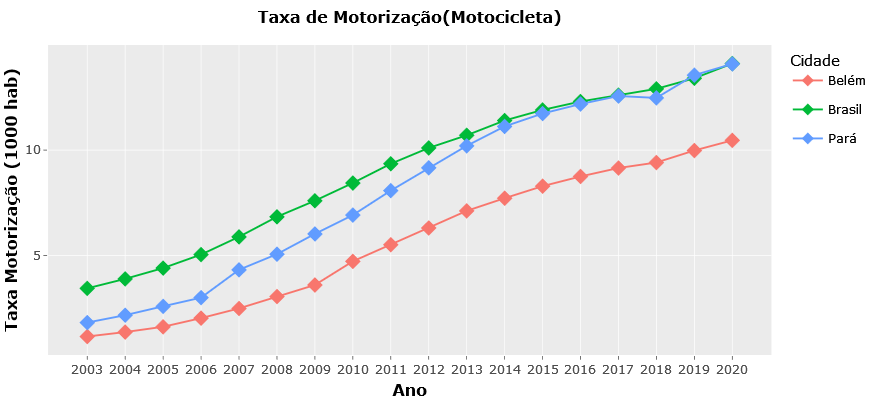
\includegraphics[scale=0.5,height=200pt,width=14cm]{figures/newplot.png}
%    \caption{\textbf{(Gráfico de Linha 1):} Taxa de Motorização do Tipo Motocicleta em Belém, Pará, Brasil, no período de 2003 a 2020.}
%   \label{fig:my_label500}
%\end{figure}


%\begin{figure}[H]
%    \centering
%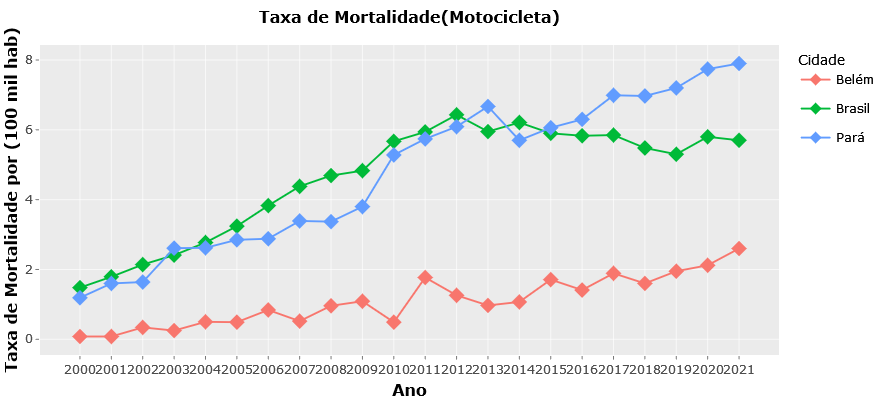
\includegraphics[scale=0.5,height=200pt,width=14cm]{figures/newplot(1).png}
%    \caption{\textbf{(Gráfico de Linha 2):} Taxa de Mortalidade na condição de Motociclista em Belém, Pará, Brasil, no período de 2002 a 2021.}
%    \label{fig:my_label500}
%\end{figure}
%%%%%%%%%%%%%%%%%%%%%%%%%%%%%%%%%%%%%%%%%%%%%%%%%%%%%%%%%%%%%%%%%%%%%%%%%%%%%%%%%%%%%%%%%%


%------------------------------------------------------------------------------------------------------%
\subsection{Gráfico Circular, Setorial ou Pizza}

O \textbf{gráfico circular}, também denominado gráfico setorial ou gráfico de
pizza (\textit{pie chart}), é utilizado para representar a distribuição de
um conjunto de dados em relação ao total. Sua principal finalidade é comparar
a participação relativa de cada categoria dentro de uma população ou amostra. \vskip0.3cm

Esse tipo de gráfico é construído a partir de um círculo dividido em setores,
cujas áreas são proporcionais aos valores observados. Assim, cada setor
representa uma parcela do total, podendo ser expresso tanto em números
absolutos quanto em percentuais. \vskip0.3cm

De forma geral, recomenda-se que:

\begin{itemize}
    \item Os setores sejam apresentados em ordem decrescente de frequência;
    \item A leitura seja feita a partir da parte superior do círculo e no sentido horário;
    \item As categorias sejam claramente identificadas, evitando excesso de informações.
\end{itemize}

Apesar de sua popularidade, a utilização do gráfico de setores deve ser feita
com cautela. Seu uso é \textbf{desaconselhado} quando:

\begin{itemize}
    \item Deseja-se comparar mais de um período temporal;
    \item Há muitas categorias (mais de cinco);
    \item As categorias possuem valores muito próximos, dificultando a distinção visual.
\end{itemize}

Nessas situações, a principal função do gráfico --- a comparação --- pode ser
prejudicada, sendo geralmente preferível substituí-lo por um gráfico de barras
ou colunas. \vskip0.3cm

Além disso, quando a variável analisada é do tipo \textbf{ordinal}, gráficos
de colunas são mais adequados, pois permitem preservar a ordem natural das
categorias, facilitando a interpretação (BARBETA, 2010).
%------------------------------------------------------------------------------------------------------%


\subsubsection{Gráfico de Rosca (\textit{Donut Chart})}

O \textbf{gráfico de rosca}, também conhecido como gráfico de rosquinha
(\textit{donut chart}), é uma variação moderna do gráfico circular ou gráfico
de pizza. Sua principal característica é a presença de um espaço vazio no
centro, formando uma estrutura semelhante a uma rosca. \vskip0.3cm

Assim como no gráfico de setores, o objetivo do gráfico de rosca é representar
a participação relativa de categorias em relação ao total. Cada segmento
corresponde a uma categoria, e o tamanho do arco (ou área) de cada pedaço
indica a proporção associada àquela classe. \vskip0.3cm

Uma vantagem estética desse tipo de gráfico é que o espaço central pode ser
utilizado para inserir informações adicionais, como o total da amostra,
percentuais globais ou descrições resumidas, tornando a visualização mais
atrativa e funcional. \vskip0.3cm

Os gráficos de rosca são frequentemente considerados uma alternativa mais
contemporânea ao gráfico de pizza, pois apresentam um design mais leve e
adaptável a diferentes estilos visuais. No entanto, as mesmas limitações
interpretativas permanecem: quando há muitas categorias ou valores muito
semelhantes, a comparação entre setores torna-se difícil. \vskip0.3cm

Além disso, em algumas situações pode-se utilizar versões reduzidas, como o
\textbf{gráfico de meia rosca}, que economiza espaço e pode ser útil em painéis
ou relatórios com muitas representações simultâneas.


%\begin{figure}[H]
%    \centering
%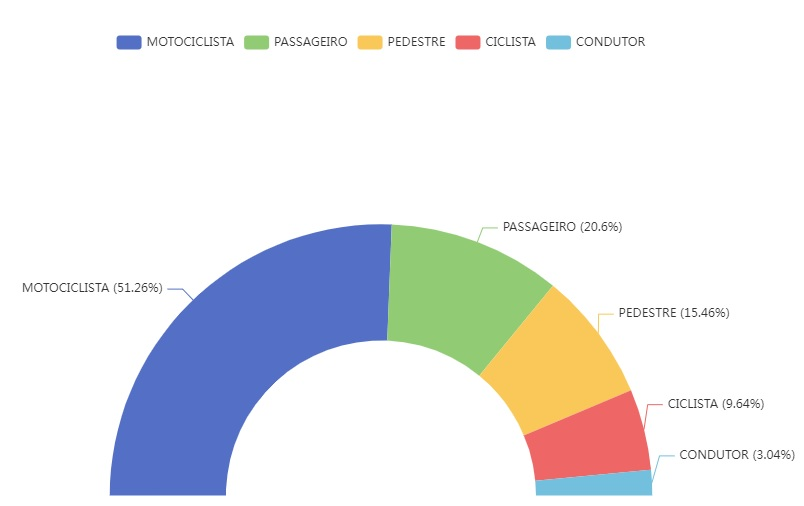
\includegraphics[scale=0.2,height=200pt,width=11cm]{figures/Rosca2.jpeg}
%    \caption{\textbf{(Gráfico Meia Rosca):} Condição das Vítimas Não Fatais por
%    Acidentes de Trânsito, registradas no município de Belém (PA), no período
%    de 2016 a 2024.}
%    \label{fig:my_label300}
%\end{figure}
%------------------------------------------------------------------------------------------------------%
\newpage
\subsection{Gráfico Radar ou Polar}

O \textbf{gráfico radar}, também chamado de \textbf{gráfico polar}, é uma forma
de representação gráfica utilizada para comparar simultaneamente três ou mais
variáveis quantitativas. Nesse tipo de gráfico, cada variável é representada
por um eixo que parte de um mesmo ponto central, formando uma estrutura
semelhante a uma teia. \vskip0.3cm

Esse formato é especialmente útil quando se deseja observar padrões gerais,
comparar perfis entre diferentes grupos ou identificar rapidamente quais
dimensões apresentam maiores ou menores valores em relação às demais. \vskip0.3cm

Entretanto, a interpretação de gráficos radar exige maior atenção do leitor,
pois a sobreposição de áreas e a disposição circular podem dificultar a
comparação precisa entre categorias, principalmente quando há muitas variáveis
ou valores muito próximos. \vskip0.3cm

O gráfico radar é também conhecido por diversas outras denominações, como
\textbf{gráfico de teia}, \textbf{gráfico de aranha}, \textbf{gráfico estrela},
\textbf{polígono irregular}, \textbf{diagrama polar} ou ainda
\textbf{diagrama Kiviat} (Mosley e Mayer, 1999).

%\begin{figure}[H]
%    \centering
%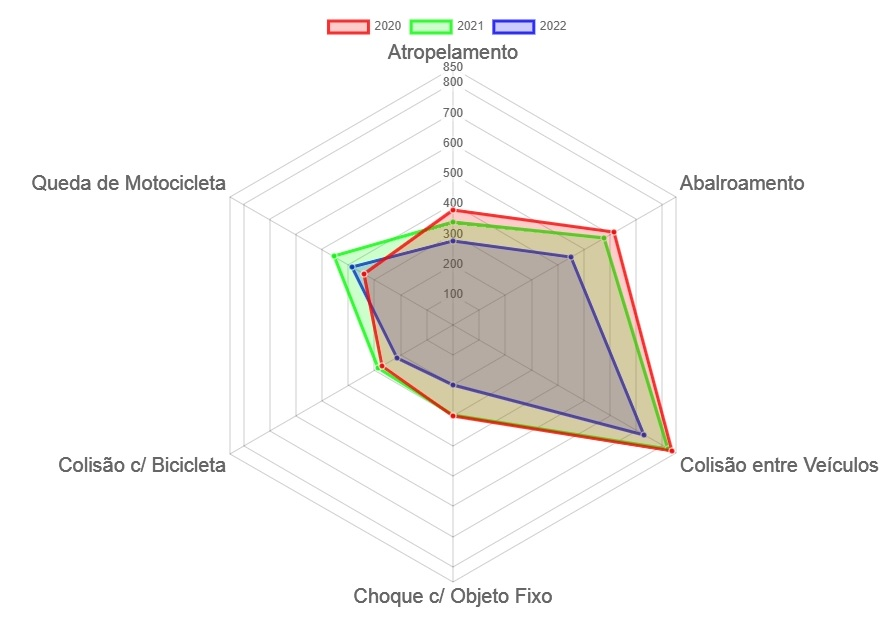
\includegraphics[scale=0.25,height=260pt,width=12cm]{figures/radarplot1.jpeg}
%    \caption{Acidentes de Trânsito por Tipo, registrados no município de Belém,
%    Estado do Pará, no período de 2020 a 2022.}
%    \label{fig:my_label30}
%\end{figure}

%------------------------------------------------------------------------------------------------------%
\newpage
\subsection{Gráfico em Pirâmide Etária}

A \textbf{pirâmide etária} é um tipo particular de histograma amplamente
utilizado em análises demográficas, pois permite visualizar, em uma única
representação gráfica, a distribuição da população por faixas de idade e,
simultaneamente, comparar essa distribuição entre os gêneros. \vskip0.3cm

Esse gráfico é especialmente importante para o estudo da estrutura populacional,
uma vez que evidencia características como o envelhecimento da população,
o predomínio de determinados grupos etários e possíveis desequilíbrios entre
homens e mulheres. \vskip0.3cm

Quando construída com valores absolutos, a pirâmide fornece uma noção clara da
dimensão populacional. Contudo, essa forma de apresentação dificulta comparações
entre diferentes regiões ou períodos históricos. Para comparações no espaço e
no tempo, recomenda-se utilizar valores relativos (percentuais), tornando os
gráficos mais comparáveis (NAZARETH, 1996). \vskip0.3cm

A pirâmide etária representa a estrutura da população segundo \textbf{idade} e
\textbf{sexo}. O eixo vertical apresenta os grupos etários, geralmente organizados
em intervalos de cinco anos, embora também possam ser utilizados intervalos anuais.
O eixo horizontal indica o tamanho do contingente populacional, em termos absolutos
ou relativos. \vskip0.3cm

Convencionalmente, o lado esquerdo do gráfico é destinado à representação da
população masculina, enquanto o lado direito representa a população feminina.
Essa disposição facilita a comparação visual entre os gêneros em cada faixa etária. \vskip0.3cm

A análise da forma da pirâmide pode revelar padrões demográficos relevantes:
pirâmides com base larga indicam populações jovens e elevadas taxas de natalidade,
enquanto pirâmides com topo mais largo sugerem envelhecimento populacional e maior
expectativa de vida.


%\begin{figure}[H]
%    \centering
%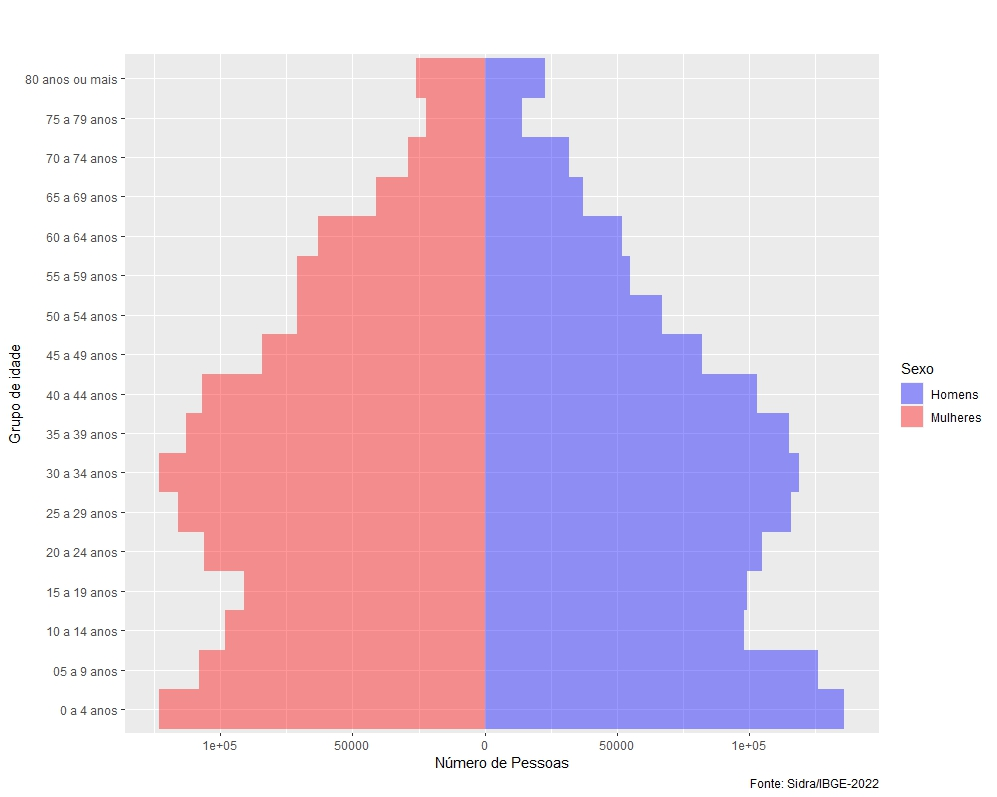
\includegraphics[scale=0.3,height=260pt,width=13cm]{figures/piramide1.jpeg}
%    \caption{Pirâmide Etária da População Residente, segundo Faixa Etária no Município de Belém, Estado do Pará - 2024.}
%    \label{fig:my_label30}
%\end{figure}

%------------------------------------------------------------------------------------------------------%
\newpage
\subsection{Gráfico em Cartograma}

O \textbf{cartograma} é uma forma de representação estatística sobre uma carta
geográfica, isto é, sobre um mapa. Trata-se de um recurso gráfico empregado quando
o objetivo é apresentar dados diretamente associados a áreas territoriais,
como municípios, estados, regiões ou países. \vskip0.3cm

Também conhecido em algumas referências como \textbf{mapa estatístico} ou
\textbf{mapa temático}, o cartograma permite visualizar a distribuição espacial
de um fenômeno, facilitando a identificação de padrões geográficos, desigualdades
regionais e concentrações de determinados eventos. \vskip0.3cm

Esse tipo de gráfico é especialmente útil em estudos relacionados à saúde pública,
demografia, economia, segurança e mobilidade, pois permite analisar como os valores
de uma variável se comportam ao longo do território. \vskip0.3cm

Os cartogramas representam as quantidades correspondentes a cada divisão geográfica
por meio de elementos visuais, sendo o uso de \textbf{cores} e suas tonalidades uma
das técnicas mais comuns. Em geral, aplica-se uma escala de intensidade crescente,
na qual valores menores são associados a tons mais claros e valores maiores a tons
mais escuros, garantindo uma leitura coerente e proporcional dos dados. \vskip0.3cm

Dessa forma, os cartogramas podem expressar valores absolutos (como número total de
acidentes em cada município) ou valores relativos (como taxas por 100 mil habitantes),
sendo estes últimos mais indicados quando se deseja comparar regiões com populações
de tamanhos diferentes. \vskip0.3cm

Portanto, o cartograma constitui uma ferramenta essencial para integrar estatística
e geografia, permitindo que informações numéricas sejam interpretadas de maneira
visual e contextualizada no espaço.




%\begin{figure}[H]
%    \centering
%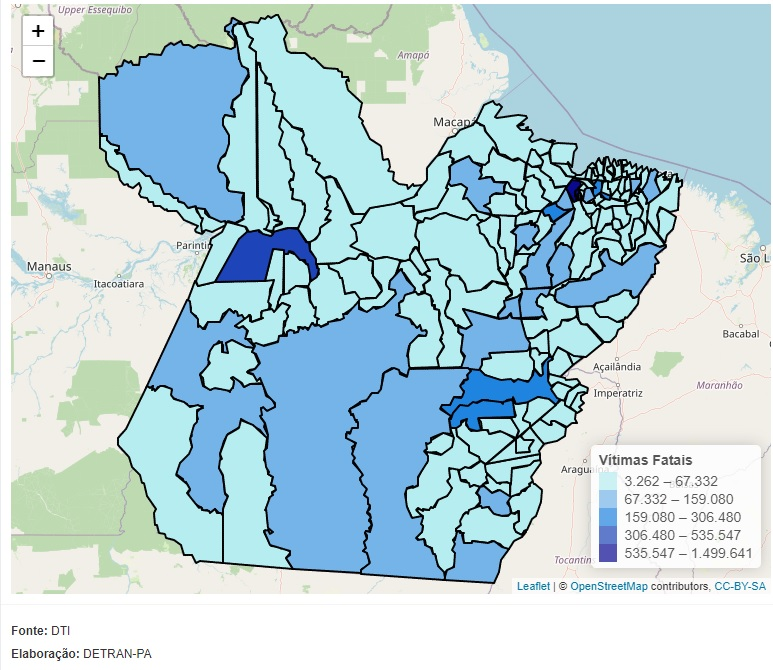
\includegraphics[scale=0.25,height=270pt,width=12cm]{figures/Map1.jpeg}
%    \caption{Vítimas Fatais por Acidentes de Trânsito, Municípios do Estado do Pará em 2024.}
%    \label{fig:my_label25}
%\end{figure}




%------------------------------------------------------------------------------------------------------%
\newpage
\subsection{Gráfico em Pictograma}

O \textbf{pictograma}, também chamado de \textbf{gráfico simbólico} ou
\textbf{gráfico ilustrativo}, é uma forma de representação estatística
baseada no uso de figuras ou ícones que simbolizam determinado fenômeno.
Esse tipo de gráfico destaca-se por sua apresentação visualmente atrativa,
sendo capaz de comunicar informações de maneira rápida e intuitiva ao público. \vskip0.3cm

Em um pictograma, os valores estatísticos são representados por símbolos
repetidos, de modo que a quantidade de figuras corresponda, de forma
aproximada, à magnitude do dado apresentado. Assim, um ícone pode equivaler,
por exemplo, a 10 unidades, 100 pessoas ou 1.000 ocorrências, dependendo do
contexto do estudo. \vskip0.3cm

Por sua natureza essencialmente ilustrativa, o pictograma não tem como
objetivo fornecer elevada precisão numérica. Sua principal função é
\textbf{facilitar a compreensão e despertar o interesse do leitor},
razão pela qual é amplamente utilizado em materiais informativos,
revistas, campanhas educativas e publicidades, especialmente em áreas como
saúde pública e segurança no trânsito. Entretanto, devido à sua limitação em termos de rigor e detalhamento,
os pictogramas não são recomendados em trabalhos científicos ou relatórios
técnicos que exijam medidas exatas e comparações estatísticas refinadas. \vskip0.3cm

Os pictogramas mais comuns são construídos segundo o critério da repetição
de símbolos, em que a variação da quantidade de ícones é proporcional à
variação da variável representada. Essa abordagem permite uma comparação
visual simples, embora apenas aproximada.  \vskip0.3cm


\textbf{Regras Fundamentais para a Construção de um Pictograma}

\begin{enumerate}
    \item Os símbolos utilizados devem ser autoexplicativos, isto é,
    facilmente compreendidos sem necessidade de interpretações complexas;
    \item Quantidades maiores devem ser representadas pelo aumento do
    número de símbolos e não pelo aumento do tamanho de um único símbolo,
    evitando distorções visuais;
    \item O pictograma deve ser empregado para comparações gerais,
    e não para transmitir detalhes minuciosos ou valores exatos;
    \item Gráficos pictóricos devem ser utilizados como recurso ilustrativo,
    nunca como base para afirmações estatísticas rigorosas ou isoladas.
\end{enumerate}

%\newpage
%\begin{figure}[H]
%    \centering
%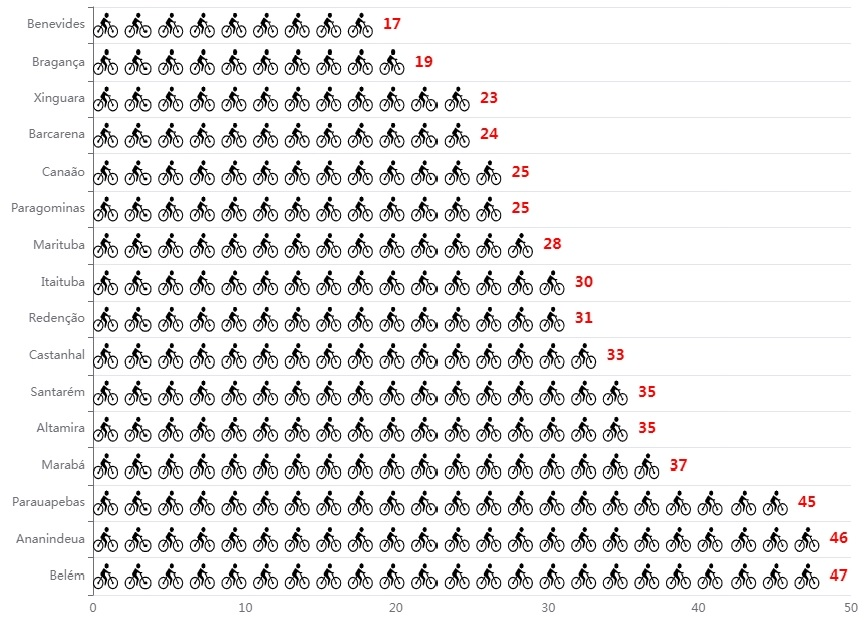
\includegraphics[scale=0.25,height=230pt,width=12cm]{figures/pictograma1.jpeg}
%\vspace{-0.5cm}
%    \caption{Pictograma de Vítimas Fatais por Sinistros de Trânsito com Bicicleta, em alguns Municípios do Estado do Pará - 2024.}
%    \label{fig:my_label50}
%\end{figure}

%\vspace{-0.7cm}
%\begin{figure}[H]
%    \centering
%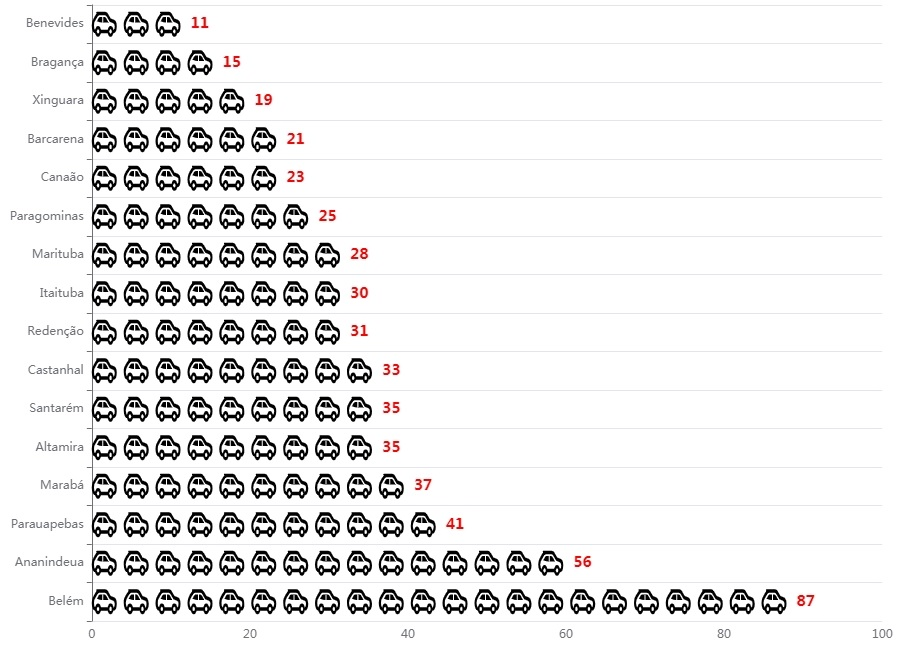
\includegraphics[scale=0.25,height=230pt,width=12cm]{figures/pictograma2.jpeg}
%\vspace{-0.5cm}
%    \caption{Pictograma de Vítimas Fatais por Sinistros de Trânsito com Automóvel em alguns Municípios do Estado do Pará - 2024.}
%    \label{fig:my_label51}
%\end{figure}



%------------------------------------------------------------------------------------------------------%

\subsection{Gráfico em Diagrama de Caixa}

John Wilder Tukey nasceu em 1915, em New Bedford (Massachusetts), numa cidade pesqueira na costa de \textit{New Jersey}. Criado em um ambiente a\-ca\-dê\-mi\-co e científico, Tukey demonstrou desde cedo um talento para a matemática e a estatística.\vskip0.3cm

\vspace{-0.2cm}
\begin{figure}
    \centering
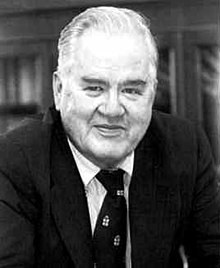
\includegraphics[scale=0.75]{figures/John_Tukey.jpeg}
    \caption{John Wilder Tukey (1915-2000)}
    \label{fig:my_label25}
\end{figure}

Tukey, graduou-se em ciências em 1936 e em química em 1937 pela \textbf{Universidade de Brown}. Posteriormente, ele continuou seus estudos na \textbf{Universidade de Princeton}, onde obteve um Ph.D. em matemática. \vskip0.3cm

Seu trabalho em estatística teve um impacto significativo, especialmente no desenvolvimento de técnicas estatísticas robustas e na análise exploratória de dados.\vskip0.3cm

Em 1977, Tukey propôs um dispositivo visual útil para a comunicação de características de uma série de dados que se tornou bastante famoso. Conhecido enormemente no meio acadêmico como Diagrama de Caixa ou Box-Plot, na qual é um tipo de gráfico que objetiva apresentar diversas informações sobre o comportamento dos dados e ainda manter uma forma compacta. \vskip0.3cm


\newpage
Na análise das informações, pode ser importante a construção de um diagrama em caixa, contendo as seguintes informações: valores mínimos e máximos, a mediana, o primeiro e o terceiro quartil, na qual representa 25\% e 75\% d  distribuição de freqüência.\vskip0.3cm


\begin{figure}[H]
\centering{
 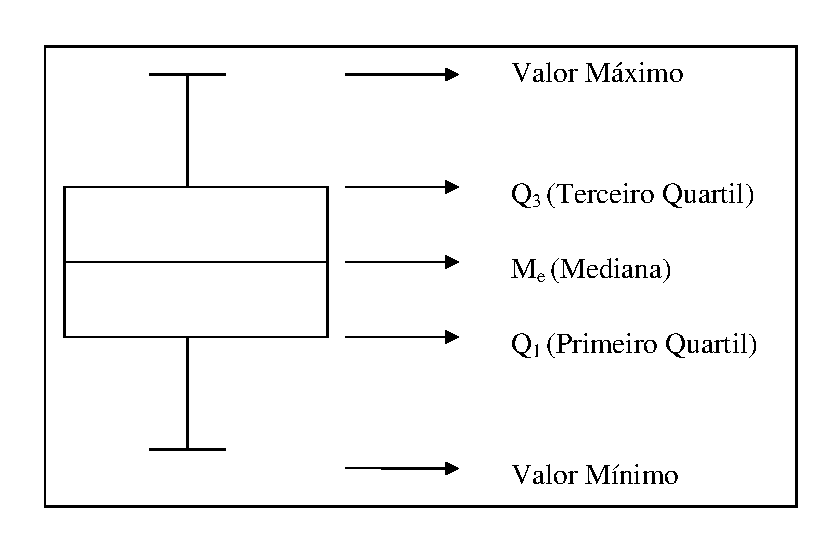
\includegraphics[scale=0.7]{figures/Boxcaixa.eps}\\
  \vspace{-0.2cm}
  \caption{Esquema Geral sobre o diagrama de caixas ou Box Plot.}\label{esquematabela}
  }
\end{figure}


As linhas verticais que saem do diagrama foram chamadas whiskers por Tukey, essas linhas servem de elo entre os valores mais centrais e os extremos da série de dados, geralmente representam os valores mínimos e máximos.\vskip0.3cm 

A mediana da série é representada por uma linha horizontal central no diagrama, e o quartil inferior (Q1) e superior (Q3), pelas linhas inferior e superior que delimitam a caixa.\vskip0.3cm  

A mediana representa uma estimativa de tendência central, e a altura da do diagrama, uma estimativa da variabilidade geral dos dados. Na qual a posição da mediana, seja ela central ou mais próxima a um dos quartis, indica a presença ou não de assimetria nos dados.\vskip0.3cm

Ao explorar um conjunto de dados de forma gráfica, deve-se considerar os valores discrepantes ou Outliers, pois eles podem revelar importantes informações e podem afetar grandemente os valores da média e do desvio-padrão, bem como disfarçar seriamente um histograma, ou seja,, um outlier pode ter efeito um dramá\-tico sobre a escala do gráfico, de modo que a verdadeira natureza da distribuição pode ser totalmente  obscurecida.


%\newpage
%\vspace{-3cm}
%\begin{figure}[H]
%    \centering
%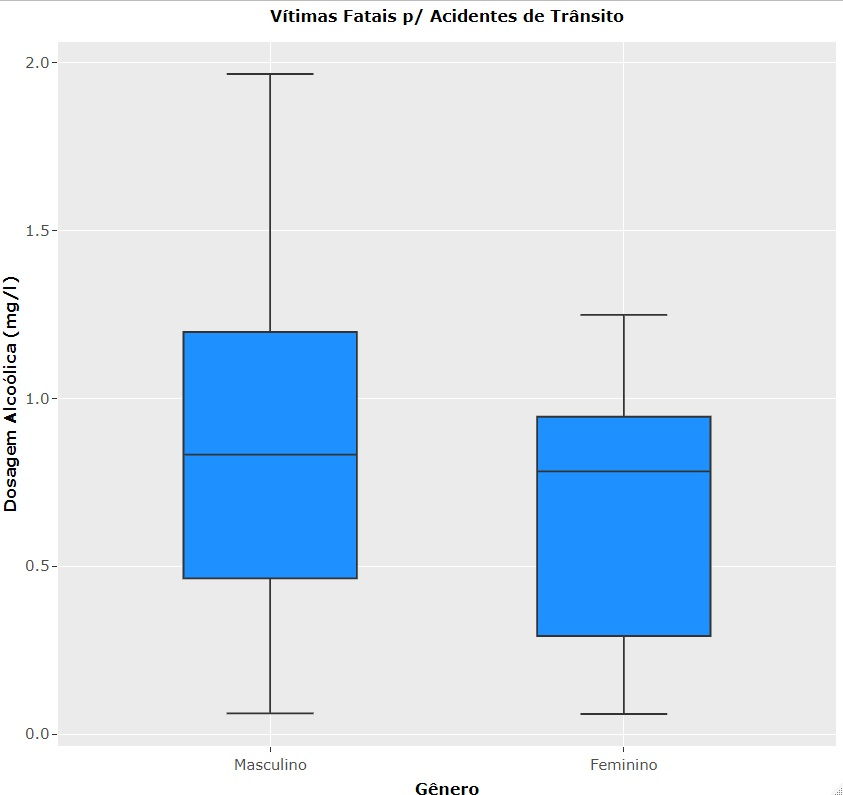
\includegraphics[scale=0.26,height=220pt,width=12cm]{figures/boxplot_dosagem.jpeg}
%    \caption{\textbf{BoxPlot Tradicional}: Dosagem Alcoólica de Vítimas Fatais por Acidentes de Trânsito, Região Metropolitrana de Belém em 2024.}
%    \label{fig:my_label25}
%\end{figure}

%\vspace{-0.7cm}
%\begin{figure}[H]
%    \centering
%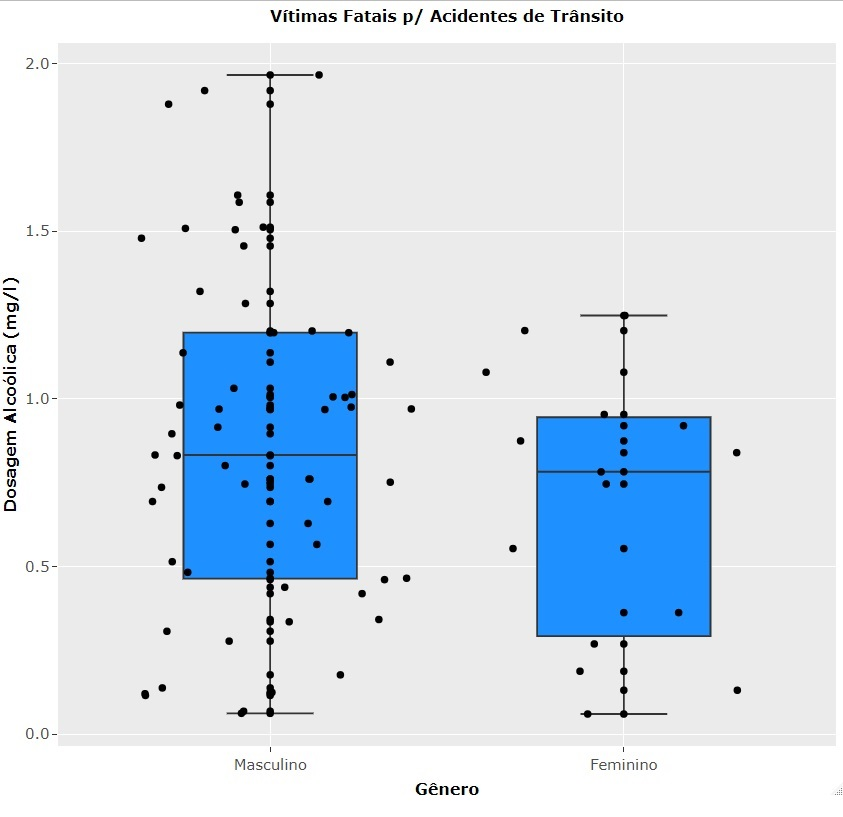
\includegraphics[scale=0.26,height=220pt,width=12cm]{figures/boxplot_dosagem_jitter.jpeg}
%    \caption{\textbf{BoxPlot com Efeito Jitter}: Dosagem Alcoólica de Vítimas Fatais por Acidentes de Trânsito, Região Metropolitrana de Belém em 2024.}
%    \label{fig:my_label25}
%\end{figure}

%------------------------------------------------------------------------------------------------------%
\subsection{Gráfico de Violino}

O \textbf{gráfico de violino} (\textit{violin plot}) é uma ferramenta
estatística moderna amplamente utilizada para representar a distribuição de uma
variável quantitativa de forma mais rica do que o boxplot tradicional. O violino pode ser entendido como uma combinação entre o \textbf{histograma} e o \textbf{boxplot}, pois reúne, em uma única visualização,
informações sobre:

\begin{itemize}
    \item a posição central dos dados (mediana);
    \item a dispersão (quartis e amplitude interquartílica);
    \item e principalmente a \textbf{densidade de probabilidade} da distribuição.
\end{itemize}

O conceito do gráfico de violino foi introduzido originalmente pelo estatístico
\textbf{Jerry L. Hintze} e pelo pesquisador \textbf{Ray D. Nelson}, no artigo
clássico publicado em 1998, como uma alternativa gráfica que permite observar
detalhadamente o formato da distribuição dos dados, indo além das limitações do
boxplot (HINTZE, 1998).
\vskip0.3cm

A forma característica do violino é construída a partir de uma estimativa
suavizada da densidade dos dados, baseada em métodos de \textbf{estimação de
densidade kernel}, cuja formulação moderna é atribuída a trabalhos fundamentais
como os de \textbf{Rosenblatt} (1956) e \textbf{Parzen} (1962). Assim, regiões
mais largas indicam maior concentração de observações, enquanto regiões mais
estreitas indicam menor frequência de valores naquele intervalo. \vskip0.3cm

De modo geral, quanto menor for o desvio padrão, mais concentrados estarão os
dados em torno da média, o que se reflete em um violino mais estreito e compacto.
Por outro lado, distribuições com maior variabilidade produzem violinos mais
alongados e largos. \vskip0.3cm

A principal vantagem do \textbf{ViolinPlot} é que ele preserva todas as
informações fornecidas pelo boxplot, mas acrescenta uma visão detalhada do
formato da distribuição, permitindo identificar assimetrias, multimodalidade
(presença de mais de um pico) e padrões que não são facilmente percebidos apenas
com o boxplot (WILKINSON, 2005).
\vskip0.3cm

Além disso, é comum adicionar ao gráfico de violino pontos individuais
representando as observações, com um pequeno deslocamento aleatório chamado de
\textbf{efeito jitter}. Essa variação facilita a visualização da dispersão real
dos dados e evita sobreposição excessiva de pontos, recurso frequentemente usado
em visualização estatística moderna (CLEVELAND, 1993).




%------------------------------------------------------------------------------------------------------%









%\vspace{-0.7cm}
%\begin{figure}[H]
%    \centering
%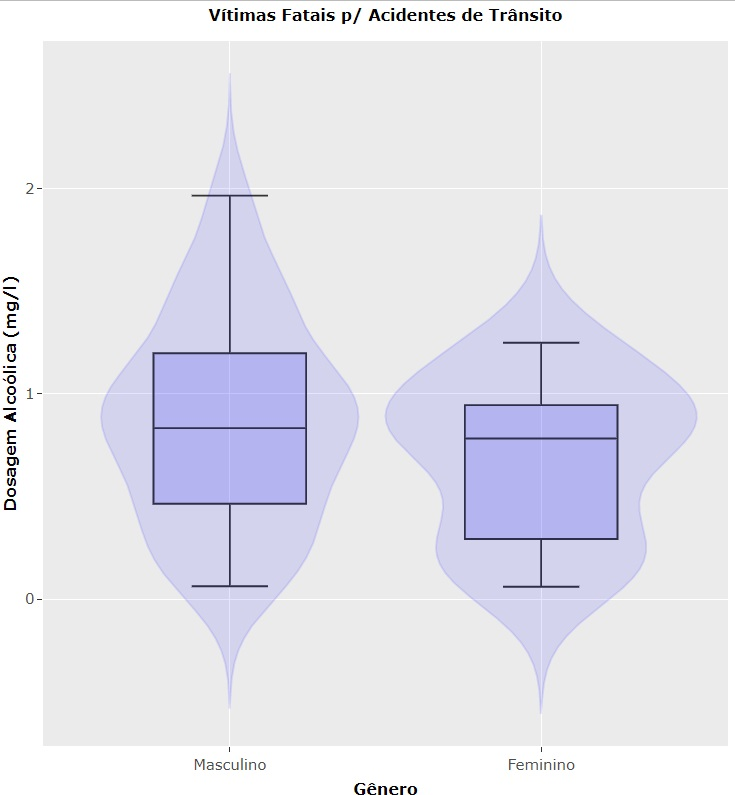
\includegraphics[scale=0.19,height=160pt,width=11cm]{figures/violinplot_Tradicional.jpeg}
%    \caption{\textbf{ViolinoPlot com BoxPlot Tradicional}: Dosagem Alcoólica de Vítimas Fatais por Acidentes de Trânsito, Região Metropolitrana de Belém em 2024.}
%    \label{fig:my_label25}
%\end{figure}

%\vspace{-0.7cm}
%\begin{figure}[H]
%    \centering
%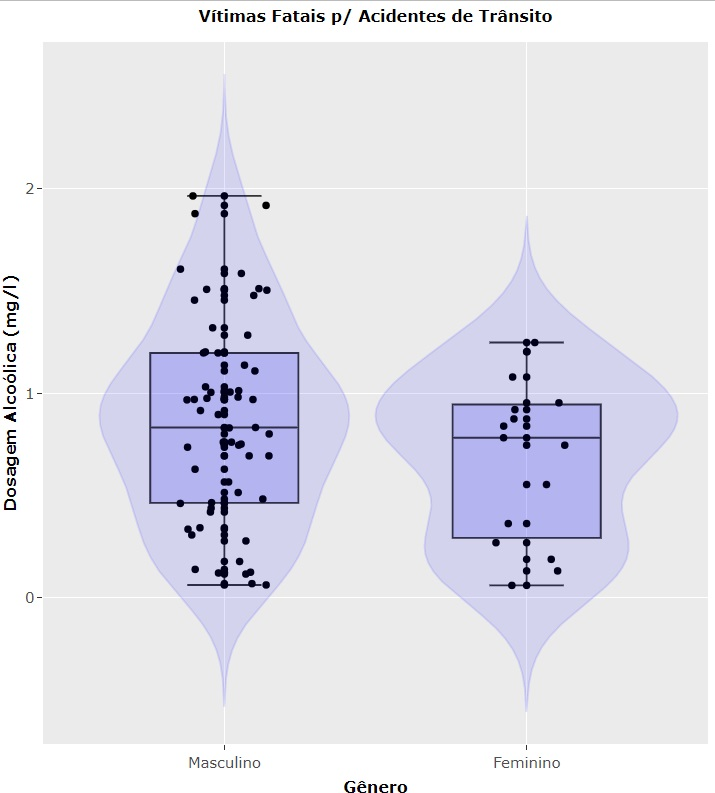
\includegraphics[scale=0.19,height=160pt,width=11cm]{figures/violinplot_jitter.jpeg}
%    \caption{\textbf{ViolinoPlot com BoxPlot e Efeito Jitter}: Dosagem Alcoólica de Vítimas Fatais por Acidentes de Trânsito, Região Metropolitrana de Belém em 2024.}
%    \label{fig:my_label25}
%\end{figure}

%------------------------------------------------------------------------------------------------------%
